
\subsection{Graph reminder}

\subsubsection{Definitions}

\begin{description}
    \item[A directed graph] is tuple (V, E) where V is the set of vertices 
        and $E \in V x V$ is the set of edges.

    \item[A path] is a suite of distinct nodes $n_0, n_1, ... n_{(k-1)}$ with
        $\big(n_i, n_{(i+1)}\big)$ an
        edge for all $0 \leq i \le k-1$. 

    Node $n_0$ is the origin and node $n_{(k-1)}$ is the
        destination.

    \item[A cycle] is suite of distinct nodes  $n_0, n_1, ... n_{(k-1)}$ with
        $\big(n_i, n_{(i+1)}\% k\big)$ an edge for all $0 \leq i \le k$.
\end{description}

\subsubsection{Graph representation}

\begin{itemize}
    \item Adjacency matrix: The simples one but matrix don't take
        sparsity into account and linear time to iterate over adjacent
        nodes.

    \item Adjacency Lists

        \begin{center}
            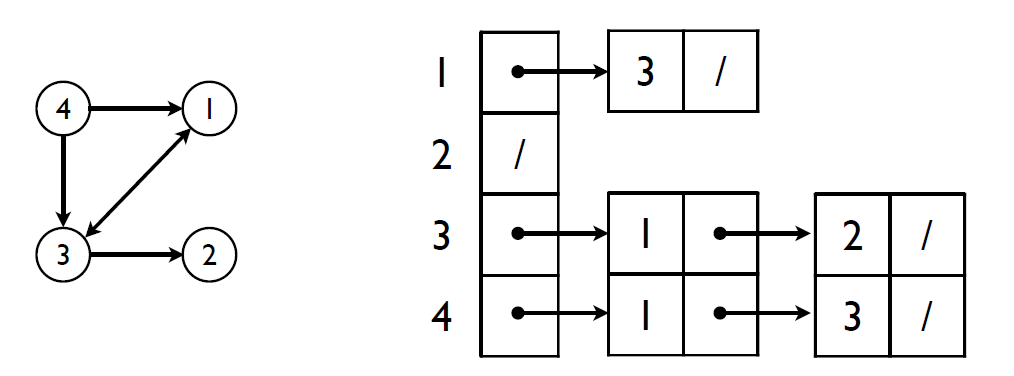
\includegraphics[width=0.3\linewidth]{AdjacencyList.png}
        \end{center}
\end{itemize}


\subsubsection{DFS}

\begin{tabular}{m{6cm}m{6cm}m{3cm}}
    \begin{lstlisting}
DFS(V , E):
    // Initialization;
    Create global variable Color[1..|V |]
    Create global variable P arent[1..|V |]
    for each node $u \in V$ do 
        Color[u] = white
        Parent[u] = Nul
    // Start the search
    for each node $U \in V$ do
        if Color[u] = white then
            Visit(u, V, E)
    \end{lstlisting}
    &
    \begin{lstlisting}
Visit(u, V, E):
    Color[u] = Grey
    for $v \in Adj[u]$ do
        // Explore arc (u, v)
        if Color[v] = white then
            Parent[v] =  u
            Visit(v, V, E)
    Color[u] = black
    \end{lstlisting}
    &
    \begin{itemize}
        \item White: Unvisited
        \item Grey: Not all adjacent edge visited
        \item Black: Fully visited
        \end{itemize}
\end{tabular}

$\Rightarrow$ Say that as we are in a graph, we need to color node that we have
already explored so that we don't reexplore them. 

\paragraph{Complexity}
\begin{itemize}
    \item Init: $O(|V|)$
    \item $O(|V| + |E|)$ : As we have to check every edges at every node
        but we pass on each node once.
\end{itemize}

\subsection{Max flow}

Max flow is a combinatorial problem on Graphs.
He can be solved in polynomial time !

\subsubsection{Definitions}

\begin{itemize}
    \item \textbf{s} is the source and \textbf{t} is the sink
    \item $c(a, b)$ is the \textbf{capacity} between nodes $a$ and $b$.
        ($c(a, b)=0$ if there isn't a edge)

    \item $f(a, b)$ is the \textbf{flow quantity} between node $a$ and
        $b$. (A flow is a vector $f$ such that each composant is associated to a
        pair of nodes.)
$$f(a,b) = -f(a,b)$$ 
\end{itemize}

An \textbf{instance of the Max Flow problem} is characterized by the
graph $G = (V, E)$, the source $s$, the sink $t$ and the vector of
capacity $c$.

\paragraph{Constraints}
\begin{itemize} 
    \item \textbf{Flow conservation} constraint: the
        quantity of water entering into a node (different from
        source and sink) is exactly the same as the quantity of of
        water exiting this node.
        \begin{eqnarray*}
            \forall a\in V\{s,t\} & 
            \sum_{b|(b,a) \in E} \quad f(b,a)  &= \sum_{b|(a,b) \in E}
            \quad f(a,b) 
        \end{eqnarray*}
        Or equivalently
        \begin{eqnarray*}
            \forall a\in V\{s,t\} & 
            \sum_{b \in V} \quad f(a,b)  &= 0
        \end{eqnarray*}

\item \textbf{Capacity} constraint: the flow through each edge does
    not exceed the capacity of this edge.
    \begin{eqnarray*}
        \forall (a,b) \in E & f(a, b) \leq c(a, b)\\
        \forall (a,b) \notin E & f(a, b) \leq 0
    \end{eqnarray*}
\end{itemize}

\paragraph{Flow}
\begin{itemize} 
    \item A \textbf{valid flow} satisfies the two constraints
    \item A \textbf{null} flow is a valid flow where $f(a,b)=0$ for each
        edge
    \item The \textbf{value of a valid flow} is the water quantity out
        of the source. Because of the conservation flow constraint, this
        value is also equal to the quantity entering the sink.
        \begin{eqnarray*}
            v(f) =    \sum_{a \in V |(s,a) \in E} \quad f(s,a)  =
            \sum_{a \in V|(a,t) \in E}
            \quad f(a,t) 
        \end{eqnarray*}

    \item[$\Rightarrow$] The max flow problem is to discover a valid flow of
maximal value
\end{itemize}



\subsubsection{Graphical representation}

\begin{tabular}{m{9cm}m{8cm}}
We usually only represent edges with positive capacity and non
negative flows. We now implicitly add the \textbf{reverse edges} with
capacity 0.
&
    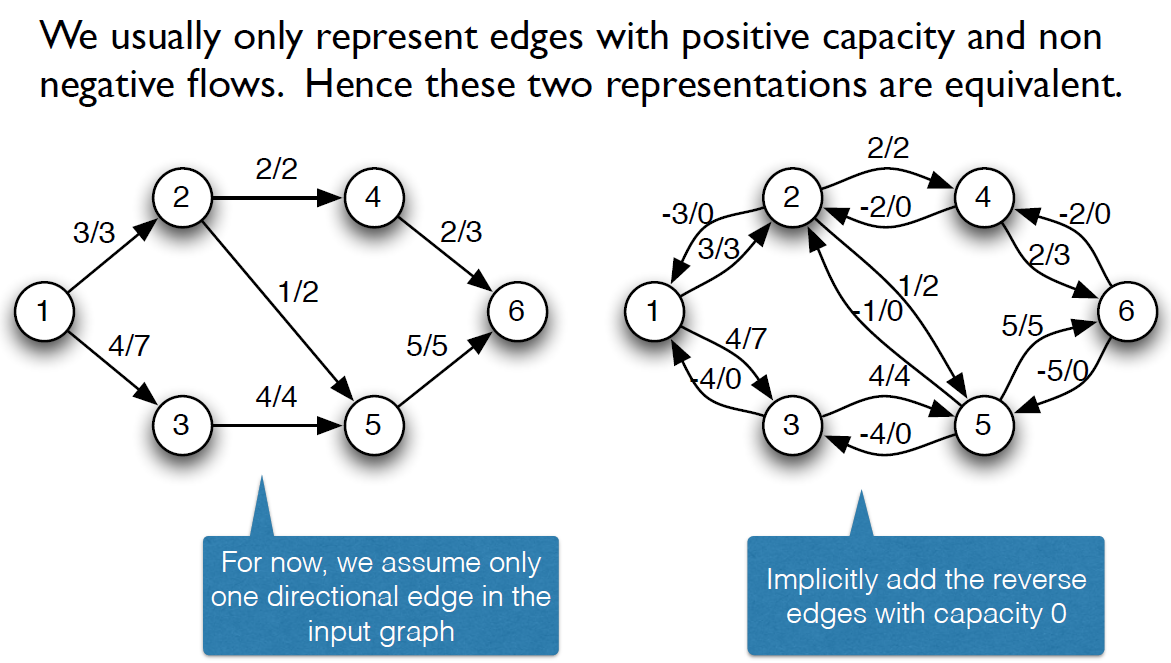
\includegraphics[width=\linewidth]{MaxFlowGraphRepr.png}
\end{tabular}

\begin{tabular}{m{10cm}m{1.5cm}m{1.5cm}}
For bidirectional edges, the reverse edge that we have will have the capacity of the second edge as shown in the example below.
&
    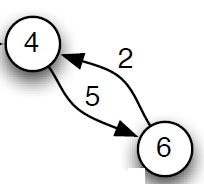
\includegraphics[width=\linewidth]{MaxFlowBidirectionnalRepresentation.png}
    &
    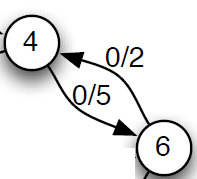
\includegraphics[width=\linewidth]{MaxFlowBidirectionnalRepresentation2.png}
\end{tabular}


\subsubsection{Residual and augmenting path}

\begin{itemize}
    \item \textbf{Residual graph} $G_f = (V, E_f)$ are used to discover paths from the
        source to the sink on which it is possible to push an
        additional quantity of water and so increase the value of the
        flow. 

        \begin{itemize}
            \item This graph is composed of exactly the same nodes as the
                original graph $G = (V, E)$ but the edges may have a different
                direction and a different (residual) capacity.

            \item A edge $(a, b)$ is in the residual only if it is not
                satured (we can add flow):
                $$(a, b) \in E_f \Leftrightarrow f(a, b) < c(a, b)$$

            \item The residual capacity is 
                $$c_f(a, b) = c(a, b) - f(a, b)$$

            \item The residual flow is
                $$f'(a, b) = \begin{cases}
                    f(a,b) + q & if (a, b) \in C\\
                    f(a,b) - q & if (b, a) \in C\\
                    f(a,b)  & otherwise\\
                \end{cases}$$
        \end{itemize}

        \begin{center}
            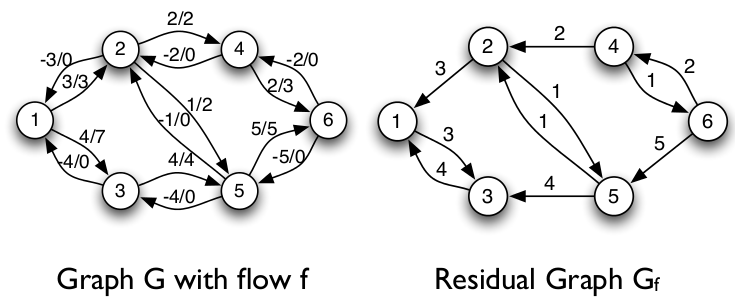
\includegraphics[width=8cm]{residualGraphExample}
            \end{center}

    \item A path joining the source $s$ to the sink $t$ in the residual
        graph $G_f$ is called \textbf{augmenting path}.
\end{itemize}


\subsubsection{Ford-Fulkerson Algorithm}

\begin{lstlisting}[mathescape]
Ford-Fulkerson(V, E, c, s, t):
// Build a vector $f$ with $\frac{|V|}{2}$ entries initialized at 0
    do
        Build the residual graph $G_f$ 
        Find a path $C$ from $s$ to $t$ in $G_f$ 
        if such a path exists then
            Let q be the smallest residual capacity on an edge of path C;
            for every edges $(a, b)$ of path $C$ do
                $f (a, b) = f (a, b) + q$
                $f (b, a) = f (b, a) q$
    while we cannot find a path between $s$ and $t$ in $G_f$ 
    return $f$ ;
\end{lstlisting}

\subsubsection{Complexity}
As the complexity of the algorithm is $O(|V| |E| U)$ with U the
maximum flow of the graph. The complexity is thus not polynomial but
pseudo-polynomial (because the input takes $log(U)$ bits to represent
$U$). For this algorithm to be polynomial you must use
delta scaling.

%TODO: sure about pseudo-code
\begin{lstlisting}
Delta-Scaling :
    delta = X > 1
    while true {
        Filter out all edges with capa < X in residual graph
        if you find an augmenting path :
            delta *= 2
            q = smallest capa of path
            for every edge of path do:
                f(a,b) = f(a,b) + q
                f(b,a) = f(b,a) - q
        else if delta > 1 :
            delta /= 2
        else
            break;
    }
    return result
\end{lstlisting}


As their are a maximum of log(U) iteration with delta scaling, the
algorithm is of polynomial complexity. The complexity becomes 
$O(|E|^2 log U)$

\begin{figure}[!ht]
    \centering
    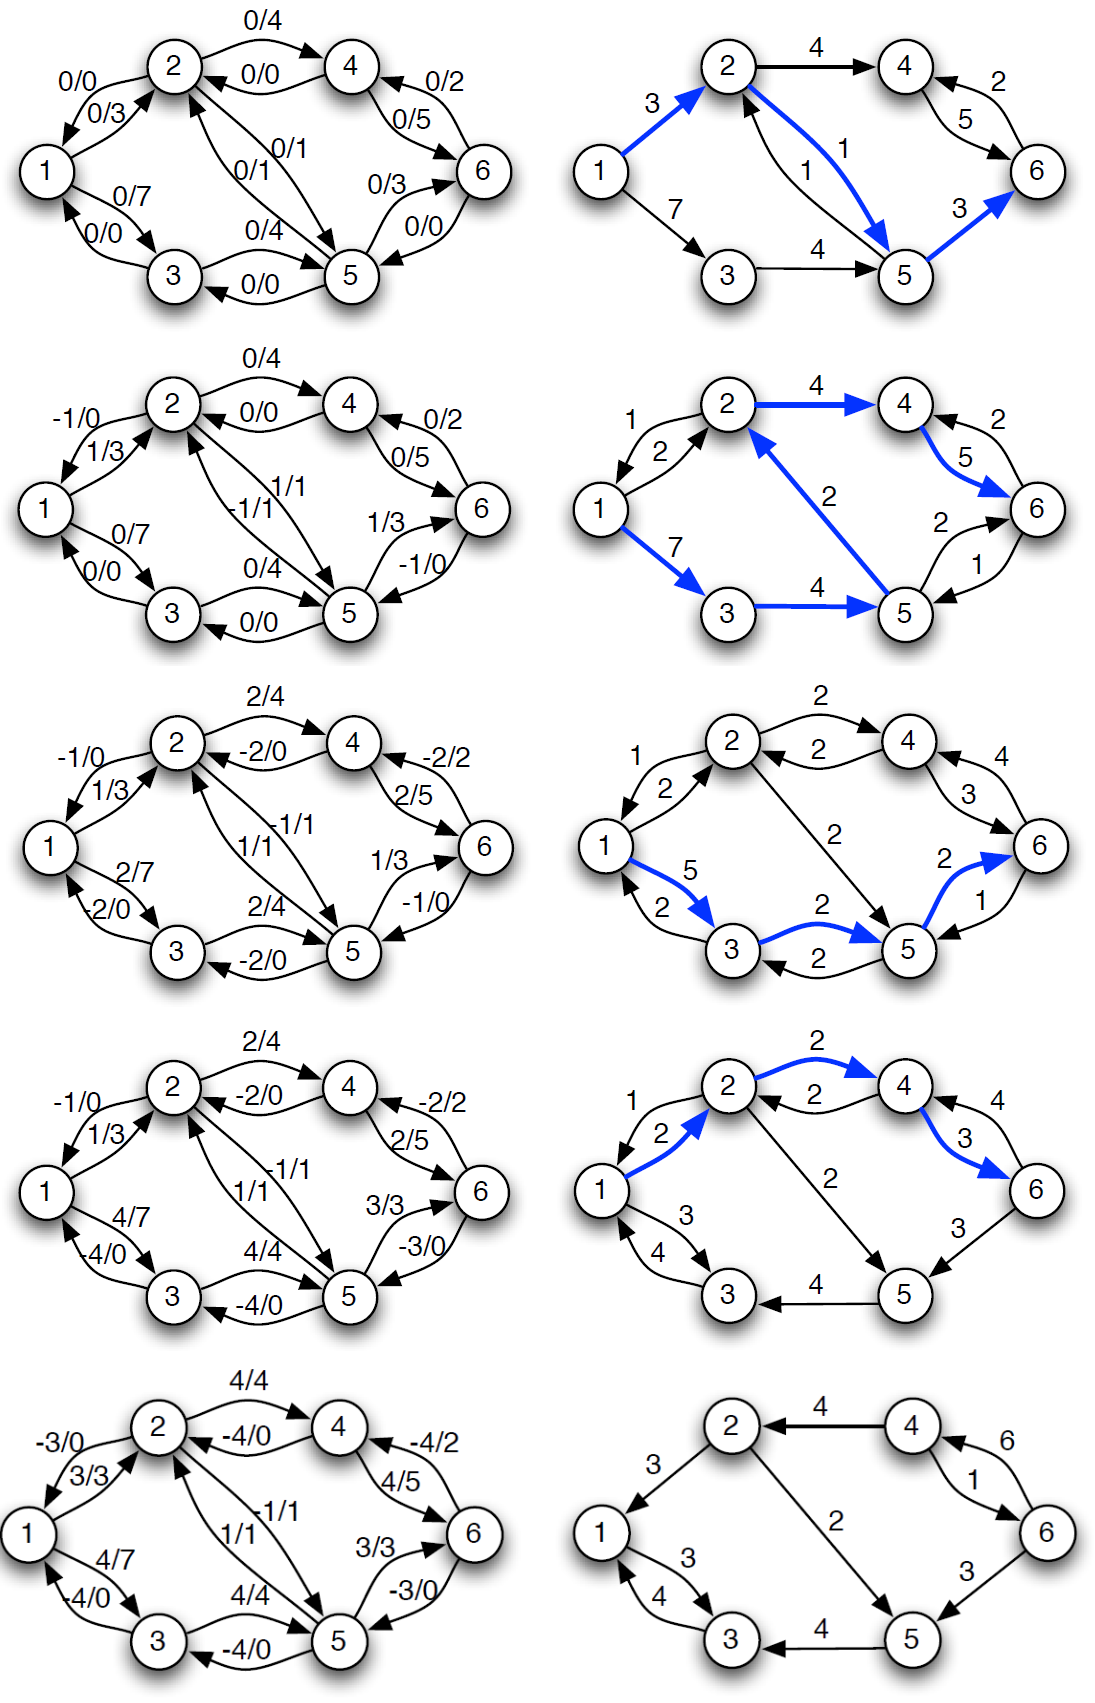
\includegraphics[width=0.55\linewidth]{MaxFlowAlgoExecutionExample.png}
    \caption{Ford-Fulkerson runtime example}
    \label{fig:Ford-Fulkerson_example}
\end{figure}


\subsection{Min cut}

How much cut do we have to make to partition a graph such that two node
$s$ and $t$, are in different partition. Answer == MaxFlow(s,t)

\subsubsection{Definitions}

\begin{itemize}
    \item A cut is bipartition of a set V formed of two disjoint sets
        $S$ and $T$ such that $V$ is the union of $S$ and $T$.
        $$S \cup T = V \quad \quad S \cap T = \emptyset $$

    \item A cut in a network is a bipartition ($S, T$) of the nodes such
        that the source is in the set $S$ and the sink is in the set $T$
        $$S \cup T = V , s\in S\quad \quad S \cap T = \emptyset, t \in
        T$$

    \item The capacity of a cut (S, T) is the capacity of the edges
        linking
        a node from S to a node in T.
        $$c(S, T) = \sum_{a\in S} \sum_{b \in T} c(a, b)$$

    \item The net flow of a cut ($S, T$) is the quantity of flow
        (positive or
        negative) from a node in S to a node in T.
        $$f(S, T) = \sum_{a\in S, b\in T} f(a, b)$$

        \begin{tabular}{m{5cm}m{6cm}}
            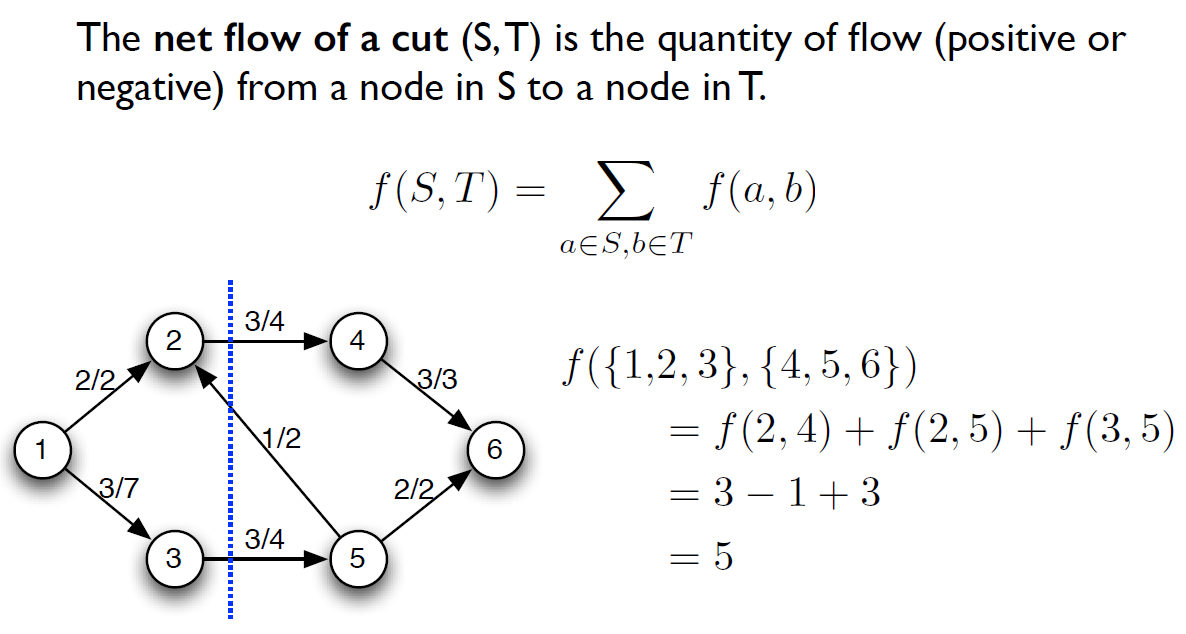
\includegraphics[width=\linewidth]{CutDefinition1.png}
            &
                \begin{eqnarray*}
                    c(\{1, 2, 3\}, \{4, 5, 6\}) & =& 8\\
                        \\
                        f(\{1,2, 3\}, \{4, 5, 6\}) & =& f(2, 4) +
                        f(2, 5) + f(3, 5)\\
                        & =& 3 - 1 + 3 \\
                        & =& 5
                    \end{eqnarray*}
        \end{tabular}
\end{itemize}


\subsubsection{Proof that min cut is solved by max flow}
%TODO ending this slide 44 for 05
\begin{figure}[!ht]
    \centering
    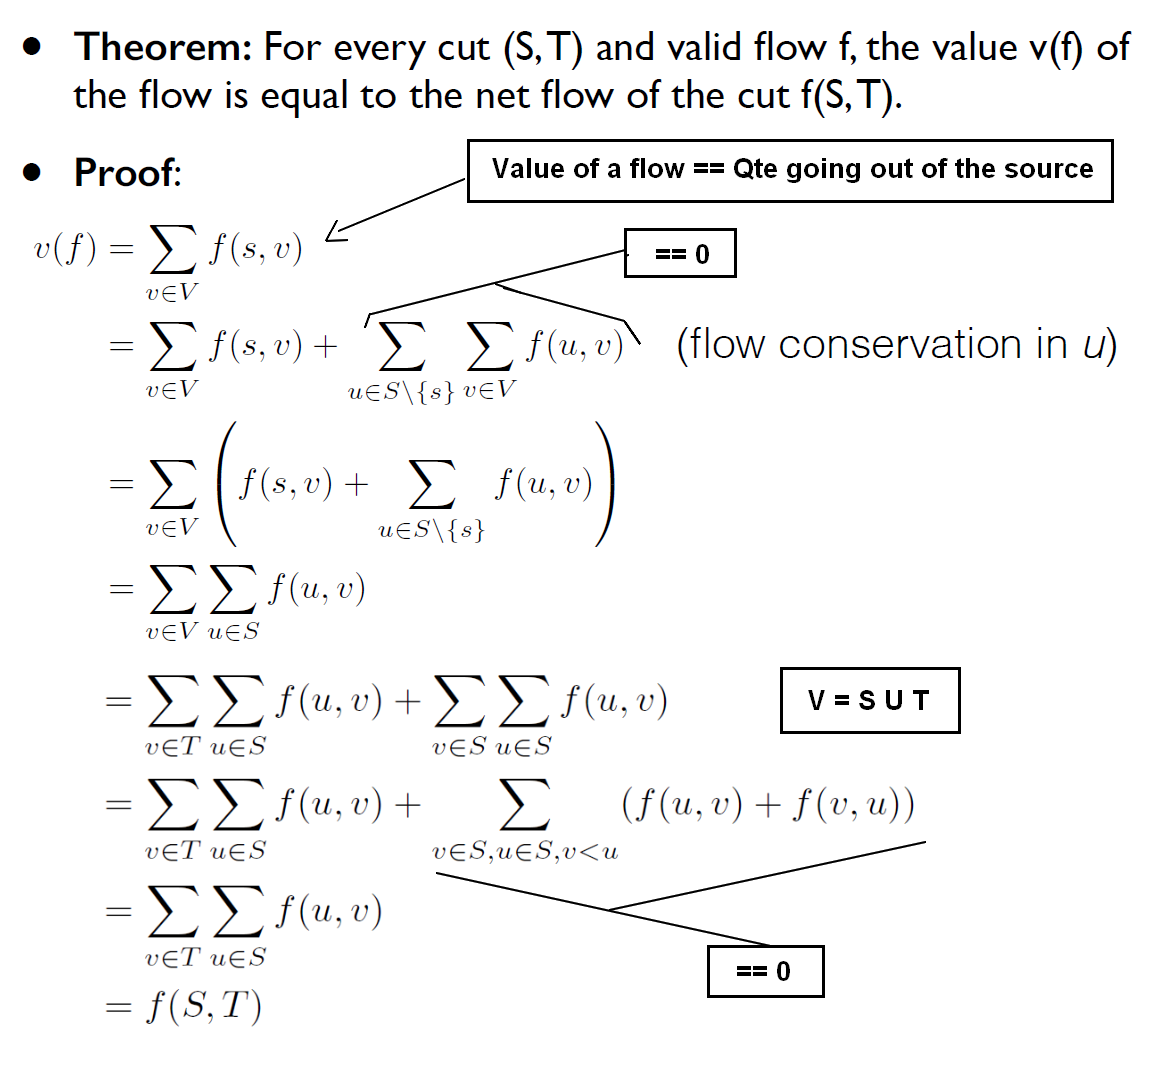
\includegraphics[width=0.7\linewidth]{CutProof.png}
\end{figure}
\FloatBarrier

\subsection{Min cost flow}
\begin{enumerate}
    \item Start with a flow of zero
    \item  Find an s-t path in G f with minimum weight
    \item  Augment along this path as much as possible (limited by
        smallest
        residual capacity of the path).
    \item  Repeat two previous steps until initial demand B of the source
        is met.
\end{enumerate}

\begin{figure}[!ht]
    \centering
    %\includegraphics[width=0.7\linewidth]{MinFlow.png}
\end{figure}

Be careful that in some problem negative weight may be used and infinite
loop must thus be avoided. => Use the Moore-Bellman-Ford algorithm
\url{https://en.wikipedia.org/wiki/Bellman%E2%80%93Ford_algorithm} 


\subsection{Scheduling}

\begin{tabular}{m{8cm}m{7cm}}
4 persons must give a seminar in a
single room with their possible slots.
\begin{itemize}
    \item  Alice (11h, 13h); Benoit (9h, 10h, 13h);
        Clotilde (9h, 11h, 13h) and Dany (11h, 13h).
\end{itemize}
&
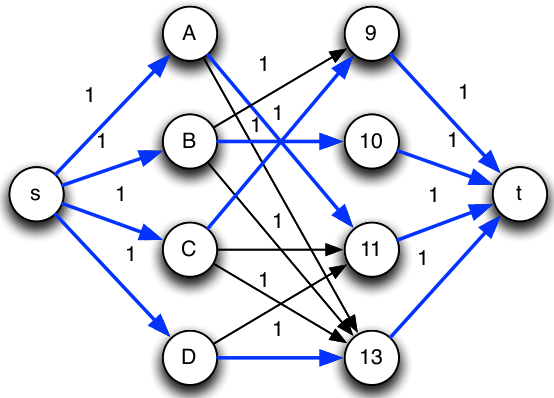
\includegraphics[width=6cm]{flowSchedul.png}
\end{tabular}



